\documentclass[12pt]{article}
\usepackage[top=1in,bottom=1in,left=1in,right=1in]{geometry}
\usepackage{alltt}
\usepackage{array}	
\usepackage{graphicx}
\usepackage{tabularx}
\usepackage{verbatim}
\usepackage{setspace}
\usepackage{listings}
\usepackage{amssymb,amsmath, amsthm}

\title{SOEN331: Introduction to Formal Methods\\for Software Engineering\\
Assignment 2 on Extended Finite State Machines}
\author{Martin Marcos 40041398,\\ Samantha Guillemette 26609198,\\ Deepkumar Patel 40096716  }

\date{\today}

\begin{document}
\begin{spacing}{1.5}

\maketitle

\newpage


\section{Driver-less car system formal specification}

\noindent The EFSM of the driver-less car system is the tuple $S = (Q, \Sigma_1, \Sigma_2, q_0, V, \Lambda)$, where\\

\noindent $Q = \{idle, parked~mode, manual~mode, cruise~mode, panic~mode, exit\}$\\

\noindent $\Sigma_1 = \{start~car, cruise~signal, drive~signal, switch, arrived, unforseen,panic~on,parked~mode~signal, panic~off, engine~off\}$\\
\noindent $\Sigma_2 = \{system~start, engine~idle, beep, system~off, stop~car, hazard~signals~on, hazard~signals~off\}$\\
\noindent $q_0: idle$\\
\noindent $V: nav~system: \{set, not~set, engine~idle, car~stopped\}$\\
\noindent $\Lambda$: Transition specifications\\
\indent 1. $\rightarrow idle$\\
\indent 2. $idle \xrightarrow {\text {start/system start; engine idle}} parked~mode$\\
\indent 3. $parked~mode  \xrightarrow {\text {engine off/system off}} exit$\\
\indent 4. $parked~mode  \xrightarrow {\text {cruise signal[not set]/beep}} manual~mode$\\
\indent 5. $parked~mode  \xrightarrow {\text {cruise signal[set]/beep}} cruise~mode$\\
\indent 6. $parked~mode  \xrightarrow {\text {drive signal[engine idle]}} manual~mode$\\
\indent 7. $manual~mode  \xrightarrow {\text {switch[set]}} cruise~mode$\\
\indent 8. $cruise~mode  \xrightarrow {\text {switch}} manual~mode$\\
\indent 9. $cruise~mode  \xrightarrow {\text {arrived}} parked~mode$\\
\indent 9. $cruise~mode  \xrightarrow {\text {unforseen/stop car; hazard signals on}} panic~mode$\\
\indent 10. $manual~mode  \xrightarrow {\text {parked mode signal[car stopped]}} parked~mode$\\
\indent 11. $panic~mode  \xrightarrow {\text {panic off/hazard signals off}} parked~mode$\\
\indent 12. $manual~mode  \xrightarrow {\text {panic~on/stop car; hazard signals on}} panic~mode$\\

\noindent The UML state diagram is shown in Figure~\ref{fig:main-system-fig}\\


\noindent As \textit{manual} is a composite state, it is defined as the tuple $S = (Q, \Sigma_1, \Sigma_2, q_0, \Lambda)$, where\\

\noindent $Q = \{running, fast, slower, break~mode, parked~mode, panic~mode\}$\\
\noindent $\Sigma_1 = \{accelerate, decelerate, break, parked~mode~signal,  panic~on, panic~off\}$\\
\noindent $\Sigma_2 = \{increase~speed, decrease~speed, 0-speed, stop~car, hazard~signal~on, hazard~signal~off\}$\\
\noindent $q_0: running$\\
\noindent $\Lambda$: Transition specifications\\
\indent 1. $\rightarrow running$\\
\indent 2. $running \xrightarrow {\text { accelerate/increase speed }} faster$\\
\indent 3. $running \xrightarrow {\text { decelerate/decrease speed }} slower$\\
\indent 4. $running \xrightarrow {\text { break/0-speed }} break~mode$\\
\indent 5. $break~mode \xrightarrow {\text { accelerate/increase speed }} running$\\
\indent 6. $faster \xrightarrow {\text { decelerate/decrease speed }} slower$\\
\indent 7. $slower \xrightarrow {\text { decelerate/decrease speed }} slower$\\
\indent 8. $slower \xrightarrow {\text { decelerate/decrease speed }} break~mode$\\
\indent 9. $break~mode \xrightarrow {\text { parked mode signal }} parked~mode$\\
\indent 10. $running \xrightarrow {\text { panic on/stop car; hazard signal on }} panic~mode$\\
\indent 11. $panic~mode \xrightarrow {\text { panic off/hazard signal off }} parked~mode$\\

\noindent The UML state diagram is shown in Figure~\ref{fig:manual-mode-fig}\\


\noindent As \textit{cruise} is a composite state, it is defined as the tuple $S = (Q, \Sigma_1, \Sigma_2, q_0, V, \Lambda)$, where\\

\noindent $Q = \{tailing~mode, changing~lane~mode, navigation~mode\}$\\
\noindent $\Sigma_1 = \{i~to~c, t~to~c, c~to~t, c~to~n, n~to~c\}$\\
\noindent $q_0: tailing~mode$\\
\noindent $\Lambda$: Transition specifications\\
\indent 1. $\rightarrow tailing~mode$\\
\indent 2. $\xrightarrow {\text{i to c}} changing~lane~mode$\\
\indent 3. $tailing~mode \xrightarrow {\text { t to c }} changing~lane~mode$\\
\indent 4. $changing~lane~mode \xrightarrow {\text { c to t }} tailing~mode$\\
\indent 5. $changing~lane~mode \xrightarrow {\text { c to n }} navigation~mode$\\
\indent 6. $navigation~mode \xrightarrow {\text { n to c }} changing~lane~mode$\\

\noindent The UML state diagram is shown in Figure~\ref{fig:cruise-mode-fig}\\


\noindent As \textit{tailing} is a composite state of \textit{cruise mode}, it is defined as the tuple $S = (Q, \Sigma_1, \Sigma_2, q_0, V, \Lambda)$, where\\

\noindent $Q = \{tailing~start, accelerate, decelerate, changing~lane~mode\}$\\
\noindent $\Sigma_1 = \{obstacle\}$\\
\noindent $\Sigma_2 = \{t~to~c, maintain~speed, switch~lane\}$\\
\noindent $q_0: tailing~start$\\
\noindent $V: speedOfCar : \{minSpeedRange, maxSpeedRange\},$\\
\indent $distanceOfCar, minSpeedRange, maxSpeedRange, minDistance: \mathbb{R} $\\
\noindent $\Lambda$: Transition specifications\\
\indent 1. $\rightarrow tailing~start$\\
\indent 2. $tailing~start\xrightarrow {\text{[s\textless minSpeedRange]}} accelerate$\\
\indent 3. $tailing~start\xrightarrow {\text{[maxSpeedRange \textless s\textgreater minSpeedRange]/t to c; maintain speed}} changing~lane~mode$\\
\indent 4. $tailing~start\xrightarrow {\text{obstacle[d\textless minDistance]/t to c; switch lane}} changing~lane~mode$\\
\indent 5. $tailing~start\xrightarrow {\text{[s\textgreater minSpeedRange or d\textless minDistance]}} decelerate$\\

\noindent The UML state diagram is shown in Figure~\ref{fig:tailing-mode-fig}\\


\noindent As \textit{changing lane} is a composite state of \textit{cruise mode}, it is defined as the tuple $S = (Q, \Sigma_1, \Sigma_2, q_0, V, \Lambda)$, where\\

\noindent $Q = \{lane~start, maintain~car~speed, tailing~mode, change~lane~mode, cruise~mode, panic~mode\}$\\
\noindent $\Sigma_1 = \{maintain~speed, switch~lane, unforseen\}$\\
\noindent $\Sigma_2 = \{c~to~t, stop~car, hazard~signal~on\}$\\
\noindent $q_0: lane~start$\\
\noindent $V: targetLane: \{car~in~t, car~not~in~t\}$,\\
\indent $speedOfCar: \{minSpeedRange, maxSpeedRange\},$\\
\indent $distanceOfCar, minSpeedRange, maxSpeedRange, minDistance: \mathbb{R} $\\
\noindent $\Lambda$: Transition specifications\\
\indent 1. $\rightarrow lane~start$\\
\indent 2. $lane~start\xrightarrow {\text{maintain speed [d\textgreater = minDistance]}} maintain~car~speed$\\
\indent 3. $maintain~car~speed\xrightarrow {\text{[d\textgreater = minDistance]}} maintain~car~speed$\\
\indent 4. $maintain~car~speed\xrightarrow {\text{[d\textless minDistance]/c to t}} tailing~mode$\\
\indent 5. $lane~start\xrightarrow {\text{maintain speed [d\textless minDistance]/c to t}} tailing~mode$\\
\indent 6. $lane~start\xrightarrow {\text{maintain speed [s\textgreater maxSpeedRange \& s\textless minSpeedRange]/c to t}} tailing~mode$\\
\indent 7. $lane~start\xrightarrow {\text{switch lane[car not in t]}} change~lane~mode$\\
\indent 8. $lane~start\xrightarrow {\text{switch lane[car in t]/c to n}} cruise~mode$\\
\indent 9. $lane~start\xrightarrow {\text{switch lane; unforseen/stop car; hazard signal on}} panic~mode$\\
\indent 10. $change~lane~mode\xrightarrow {\text{[car not in t]}} change~lane~mode$\\
\indent 11. $change~lane~mode\xrightarrow {\text{[car in t]/c to n}} cruise~mode$\\
\indent 12. $change~lane~mode\xrightarrow {\text{unforseen/stop car; hazard signal on}} panic~mode$\\

\noindent The UML state diagram is shown in Figure~\ref{fig:changing-lane-mode-fig}\\


\noindent As \textit{navigation} is a composite state of \textit{cruise mode}, it is defined as the tuple $S = (Q, \Sigma_1, \Sigma_2, q_0, V, \Lambda)$, where\\

\noindent $Q = \{navigation~start, turn~left,turn~right, turn~left~ahead, turn~right~ahead, changing~lane~mode,destination~ahead, arrived~destination\}$\\
\noindent $\Sigma_1 = \{d~on~left, d~on~right, TLA, TRA, d~ahead, car~at~d\}$\\
\noindent $\Sigma_2 = \{turn~left, turn~right, dest~ahead, car~in~t, n~to~c, switch~lane, arrived\}$\\
\noindent $q_0: navigation~start$\\
\noindent $V: targetLane: \{car~in~t, car~not~in~t\}$,\\
\noindent $\Lambda$: Transition specifications\\
\indent 1. $\rightarrow mavigation~start$\\
\indent 2. $navigation~start\xrightarrow {\text{d on left/turn left}} turn~left$\\
\indent 3. $navigation~start\xrightarrow {\text{d on right/turn right}} turn~right$\\
\indent 4. $navigation~start\xrightarrow {\text{TLA[car not in t]}} turn~left~ahead$\\
\indent 5. $navigation~start\xrightarrow {\text{TRA[car not in t]}} turn~right~ahead$\\
\indent 6. $navigation~start\xrightarrow {\text{d ahead/dest ahead; car in t}} turn~left~ahead$\\
\indent 7. $turn~left~ahead\xrightarrow {\text{/n to c; switch lane}} changing~lane~mode$\\
\indent 8. $turn~right~ahead\xrightarrow {\text{/n to c; switch lane}} changing~lane~mode$\\
\indent 9. $destination~ahead\xrightarrow {\text{car at d/arrived}} arrived~destination$\\

\noindent The UML state diagram is shown in Figure~\ref{fig:navigation-mode-fig}\\


\newpage

\section{UML state diagrams}

\begin{figure}[h!]
	\centering
		\includegraphics[width=0.8\textwidth]{./A2_Figures/A2_SOEN331_Main.eps}
		  \caption{Main System.}
  \label{fig:main-system-fig}
\end{figure}

\begin{figure}[h!]
	\centering
		\includegraphics[width=0.8\textwidth]{./A2_Figures/A2_SOEN331_Manual.eps}
		  \caption{Manual Mode.}
  \label{fig:manual-mode-fig}
\end{figure}  
   
\begin{figure}[h!]
	\centering
		\includegraphics[width=0.8\textwidth]{./A2_Figures/A2_SOEN331_Cruise.eps}
		  \caption{Cruise Mode.}
  \label{fig:cruise-mode-fig}
\end{figure}

\begin{figure}[h!]
	\centering
		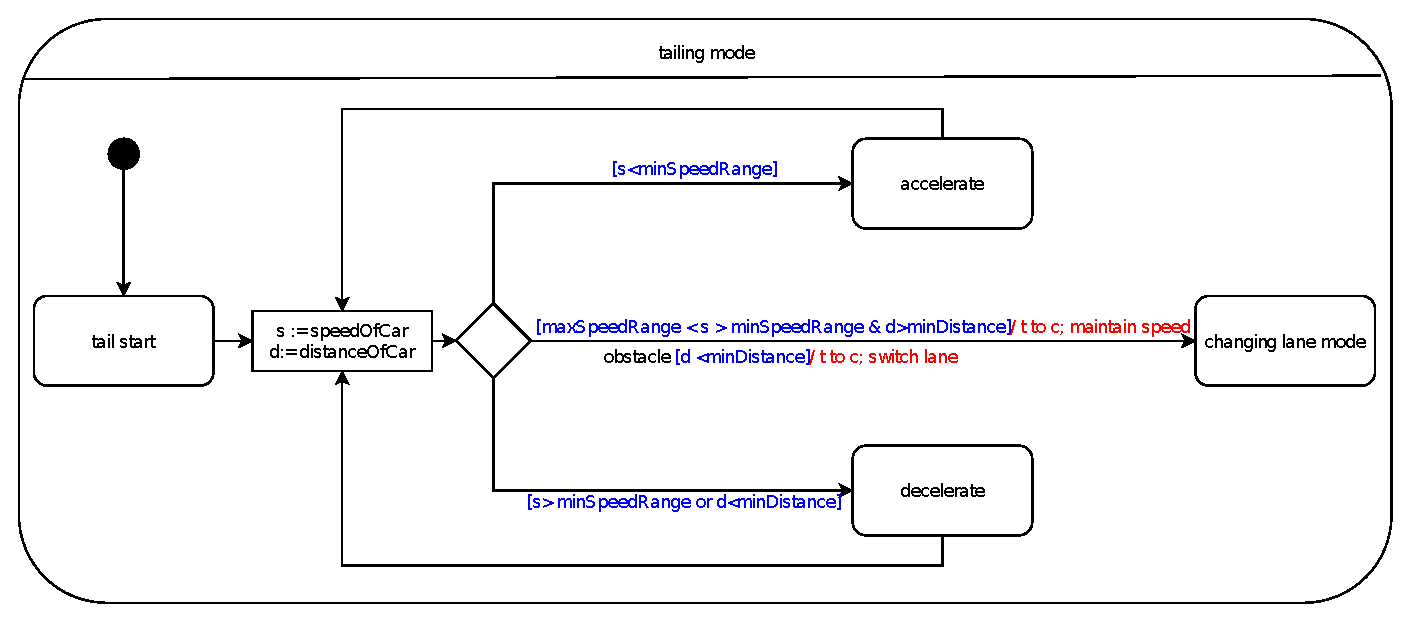
\includegraphics[width=0.8\textwidth]{./A2_Figures/A2_SOEN331_Tailing.eps}
		  \caption{Tailing Mode.}
  \label{fig:tailing-mode-fig}
\end{figure}

\begin{figure}[h!]
	\centering
		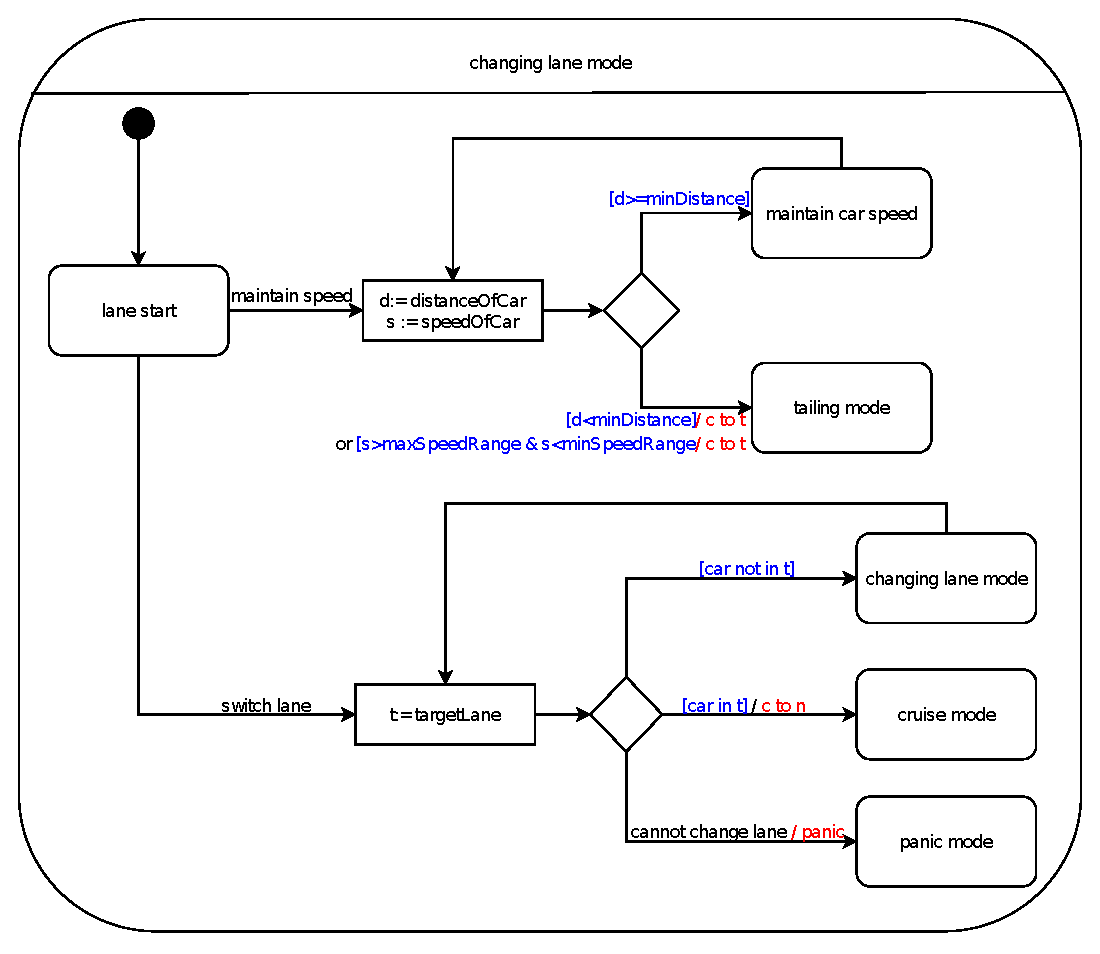
\includegraphics[width=0.8\textwidth]{./A2_Figures/A2_SOEN331_Changing_Lane.eps}
		  \caption{Changing Lane Mode.}
  \label{fig:changing-lane-mode-fig}
\end{figure}

\begin{figure}[h!]
	\centering
		\includegraphics[width=0.8\textwidth]{./A2_Figures/A2_SOEN331_Navigation.eps}
		  \caption{Navigation Mode.}
  \label{fig:navigation-mode-fig}
\end{figure}

\end{spacing}

\end{document}
